% Options for packages loaded elsewhere
\PassOptionsToPackage{unicode}{hyperref}
\PassOptionsToPackage{hyphens}{url}
%
\documentclass[
  10pt,
  ignorenonframetext,
]{beamer}
\usepackage{pgfpages}
\setbeamertemplate{caption}[numbered]
\setbeamertemplate{caption label separator}{: }
\setbeamercolor{caption name}{fg=normal text.fg}
\beamertemplatenavigationsymbolsempty
% Prevent slide breaks in the middle of a paragraph
\widowpenalties 1 10000
\raggedbottom
\setbeamertemplate{part page}{
  \centering
  \begin{beamercolorbox}[sep=16pt,center]{part title}
    \usebeamerfont{part title}\insertpart\par
  \end{beamercolorbox}
}
\setbeamertemplate{section page}{
  \centering
  \begin{beamercolorbox}[sep=12pt,center]{part title}
    \usebeamerfont{section title}\insertsection\par
  \end{beamercolorbox}
}
\setbeamertemplate{subsection page}{
  \centering
  \begin{beamercolorbox}[sep=8pt,center]{part title}
    \usebeamerfont{subsection title}\insertsubsection\par
  \end{beamercolorbox}
}
\AtBeginPart{
  \frame{\partpage}
}
\AtBeginSection{
  \ifbibliography
  \else
    \frame{\sectionpage}
  \fi
}
\AtBeginSubsection{
  \frame{\subsectionpage}
}
\usepackage{amsmath,amssymb}
\usepackage{lmodern}
\usepackage{setspace}
\usepackage{iftex}
\ifPDFTeX
  \usepackage[T1]{fontenc}
  \usepackage[utf8]{inputenc}
  \usepackage{textcomp} % provide euro and other symbols
\else % if luatex or xetex
  \usepackage{unicode-math}
  \defaultfontfeatures{Scale=MatchLowercase}
  \defaultfontfeatures[\rmfamily]{Ligatures=TeX,Scale=1}
\fi
% Use upquote if available, for straight quotes in verbatim environments
\IfFileExists{upquote.sty}{\usepackage{upquote}}{}
\IfFileExists{microtype.sty}{% use microtype if available
  \usepackage[]{microtype}
  \UseMicrotypeSet[protrusion]{basicmath} % disable protrusion for tt fonts
}{}
\makeatletter
\@ifundefined{KOMAClassName}{% if non-KOMA class
  \IfFileExists{parskip.sty}{%
    \usepackage{parskip}
  }{% else
    \setlength{\parindent}{0pt}
    \setlength{\parskip}{6pt plus 2pt minus 1pt}}
}{% if KOMA class
  \KOMAoptions{parskip=half}}
\makeatother
\usepackage{xcolor}
\geometry{left = 1cm, right = 0.5cm, top = 0.5cm, bottom = 0.5cm}
\newif\ifbibliography
\usepackage{color}
\usepackage{fancyvrb}
\newcommand{\VerbBar}{|}
\newcommand{\VERB}{\Verb[commandchars=\\\{\}]}
\DefineVerbatimEnvironment{Highlighting}{Verbatim}{commandchars=\\\{\}}
% Add ',fontsize=\small' for more characters per line
\usepackage{framed}
\definecolor{shadecolor}{RGB}{248,248,248}
\newenvironment{Shaded}{\begin{snugshade}}{\end{snugshade}}
\newcommand{\AlertTok}[1]{\textcolor[rgb]{0.94,0.16,0.16}{#1}}
\newcommand{\AnnotationTok}[1]{\textcolor[rgb]{0.56,0.35,0.01}{\textbf{\textit{#1}}}}
\newcommand{\AttributeTok}[1]{\textcolor[rgb]{0.77,0.63,0.00}{#1}}
\newcommand{\BaseNTok}[1]{\textcolor[rgb]{0.00,0.00,0.81}{#1}}
\newcommand{\BuiltInTok}[1]{#1}
\newcommand{\CharTok}[1]{\textcolor[rgb]{0.31,0.60,0.02}{#1}}
\newcommand{\CommentTok}[1]{\textcolor[rgb]{0.56,0.35,0.01}{\textit{#1}}}
\newcommand{\CommentVarTok}[1]{\textcolor[rgb]{0.56,0.35,0.01}{\textbf{\textit{#1}}}}
\newcommand{\ConstantTok}[1]{\textcolor[rgb]{0.00,0.00,0.00}{#1}}
\newcommand{\ControlFlowTok}[1]{\textcolor[rgb]{0.13,0.29,0.53}{\textbf{#1}}}
\newcommand{\DataTypeTok}[1]{\textcolor[rgb]{0.13,0.29,0.53}{#1}}
\newcommand{\DecValTok}[1]{\textcolor[rgb]{0.00,0.00,0.81}{#1}}
\newcommand{\DocumentationTok}[1]{\textcolor[rgb]{0.56,0.35,0.01}{\textbf{\textit{#1}}}}
\newcommand{\ErrorTok}[1]{\textcolor[rgb]{0.64,0.00,0.00}{\textbf{#1}}}
\newcommand{\ExtensionTok}[1]{#1}
\newcommand{\FloatTok}[1]{\textcolor[rgb]{0.00,0.00,0.81}{#1}}
\newcommand{\FunctionTok}[1]{\textcolor[rgb]{0.00,0.00,0.00}{#1}}
\newcommand{\ImportTok}[1]{#1}
\newcommand{\InformationTok}[1]{\textcolor[rgb]{0.56,0.35,0.01}{\textbf{\textit{#1}}}}
\newcommand{\KeywordTok}[1]{\textcolor[rgb]{0.13,0.29,0.53}{\textbf{#1}}}
\newcommand{\NormalTok}[1]{#1}
\newcommand{\OperatorTok}[1]{\textcolor[rgb]{0.81,0.36,0.00}{\textbf{#1}}}
\newcommand{\OtherTok}[1]{\textcolor[rgb]{0.56,0.35,0.01}{#1}}
\newcommand{\PreprocessorTok}[1]{\textcolor[rgb]{0.56,0.35,0.01}{\textit{#1}}}
\newcommand{\RegionMarkerTok}[1]{#1}
\newcommand{\SpecialCharTok}[1]{\textcolor[rgb]{0.00,0.00,0.00}{#1}}
\newcommand{\SpecialStringTok}[1]{\textcolor[rgb]{0.31,0.60,0.02}{#1}}
\newcommand{\StringTok}[1]{\textcolor[rgb]{0.31,0.60,0.02}{#1}}
\newcommand{\VariableTok}[1]{\textcolor[rgb]{0.00,0.00,0.00}{#1}}
\newcommand{\VerbatimStringTok}[1]{\textcolor[rgb]{0.31,0.60,0.02}{#1}}
\newcommand{\WarningTok}[1]{\textcolor[rgb]{0.56,0.35,0.01}{\textbf{\textit{#1}}}}
\setlength{\emergencystretch}{3em} % prevent overfull lines
\providecommand{\tightlist}{%
  \setlength{\itemsep}{0pt}\setlength{\parskip}{0pt}}
\setcounter{secnumdepth}{-\maxdimen} % remove section numbering
\usepackage{float}
\usepackage{booktabs}
\usepackage{array}
\usepackage{longtable}
\useinnertheme{rectangles}
\setbeamertemplate{itemize subitem}{\scriptsize$\diamond$}
\definecolor{blue}{RGB}{0,114,178}
\definecolor{red}{RGB}{213,94,0}
\definecolor{yellow}{RGB}{240,228,66}
\definecolor{green}{RGB}{0,158,115}
\ifLuaTeX
  \usepackage{selnolig}  % disable illegal ligatures
\fi
\IfFileExists{bookmark.sty}{\usepackage{bookmark}}{\usepackage{hyperref}}
\IfFileExists{xurl.sty}{\usepackage{xurl}}{} % add URL line breaks if available
\urlstyle{same} % disable monospaced font for URLs
\hypersetup{
  pdftitle={Introductory Statistics for Economics},
  pdfauthor={Duong Trinh},
  hidelinks,
  pdfcreator={LaTeX via pandoc}}

\title{Introductory Statistics for Economics}
\subtitle{ECON1013: LAB 2}
\author{Duong Trinh}
\date{Feb 2024}
\institute{University of Glasgow}

\begin{document}
\frame{\titlepage}

\setstretch{1.5}
\begin{frame}{Intro}
\protect\hypertarget{intro}{}
\begin{itemize}
\tightlist
\item
  Duong Trinh

  \begin{itemize}
  \tightlist
  \item
    PhD Student in Economics (Bayesian Microeconometrics)
  \item
    Email: \underline{Duong.Trinh@glasgow.ac.uk}
  \end{itemize}
\end{itemize}

\vspace{3mm}

\begin{itemize}
\tightlist
\item
  ECON1013-LB04

  \begin{itemize}
  \tightlist
  \item
    Monday 1-2 pm
  \item
    3 sessions (29-Jan, 12-Feb, 26-Feb)
  \end{itemize}
\item
  ECON1013-LB05

  \begin{itemize}
  \tightlist
  \item
    Tuesday 12-1 pm
  \item
    3 sessions (30-Jan, 13-Feb, 27-Feb)
  \end{itemize}
\item
  ECON1013-LB06

  \begin{itemize}
  \tightlist
  \item
    Tuesday 1-2 pm
  \item
    3 sessions (30-Jan, 13-Feb, 27-Feb)
  \end{itemize}
\end{itemize}

\vspace{3mm}
\end{frame}

\begin{frame}{Record Attendance}
\protect\hypertarget{record-attendance}{}
\end{frame}

\begin{frame}{Setup}
\protect\hypertarget{setup}{}
\begin{itemize}
\item
  Step 1: Download Lab materials from \textbf{Moodle} page
  \(\rightarrow\) Extract the folder in PC.
\item
  Step 2: Log in \textbf{Microsoft onedrive} using your student account
  \textcolor{blue}{https://onedrive.live.com/login/} and upload the
  folder above.
\item
  Step 3: Launch the \textbf{Excel} online
  \textcolor{blue}{https://www.office.com/launch/excel?auth=2}, which we
  will use for all lab sessions.
\end{itemize}
\end{frame}

\hypertarget{exercise-1.}{%
\section{Exercise 1.}\label{exercise-1.}}

\begin{frame}{Exercise 1.}
\begin{itemize}
\tightlist
\item
  Data set: \texttt{testscores.xls}
\item
  About: A sample (\(n=200\)) of student test scores in Math and English

  \begin{itemize}
  \tightlist
  \item
    Minimal text score is 0 and maximal test score is 100.
  \end{itemize}
\end{itemize}
\end{frame}

\begin{frame}{Part 1. Visualizing dispersion in data.}
\protect\hypertarget{part-1.-visualizing-dispersion-in-data.}{}
\begin{enumerate}
\tightlist
\item
  Plot a histogram of English test scores.
\item
  Plot a histogram of Math test scores.
\item
  Based on these two histograms, which variable do you think is more
  dispersed? (Which has a higher variance?)
\end{enumerate}
\end{frame}

\begin{frame}{Part 2. Quantifying dispersion in data.}
\protect\hypertarget{part-2.-quantifying-dispersion-in-data.}{}
\begin{enumerate}
\tightlist
\item
  Compute the mean of both test scores.
\item
  Compute the sample variance of both test scores using the Excel
  formula \textcolor{red}{VAR()}.
\item
  Compute the sample standard deviation of both test scores using Excel
  formula \textcolor{red}{STDEV()}.
\item
  Compute the variance WITHOUT using Excel formula VARIANCE. You are
  only allowed to use the Excel formulas \textcolor{red}{SUM()} and
  \textcolor{red}{COUNT()} and standard mathematics operations.
\item
  Interpret your observations. Based on the standard deviation and the
  variance, which variable is more dispersed?
\end{enumerate}
\end{frame}

\begin{frame}{Part 3. Standardizing data.}
\protect\hypertarget{part-3.-standardizing-data.}{}
\begin{enumerate}
\tightlist
\item
  For each observation of variable ``Math'' in the sample, compute the
  z-score. Use the mean and the standard deviation computed in Part 2.
\item
  Compute the mean and the standard deviation of the z-scores.
\item
  Plot the histogram of the z-scores for Math. What does the histogram
  look like?
\end{enumerate}
\end{frame}

\begin{frame}{{[}Review{]} z-score}
\protect\hypertarget{review-z-score}{}
\begin{itemize}
\item
  A z-score shows the position of a value relative to the mean of the
  distribution.
\item
  It indicates the number of standard deviations a value is from the
  mean.
\item
  If the data set is the entire population of data and the population
  mean, \(\mu\), and the population standard deviation, \(\sigma\), are
  known, then for each value, \(x_i\), the z-score associated with
  \(x_i\) is
\end{itemize}

\[
z_i = \frac{x_i - \mu}{\sigma}
\]
\end{frame}

\begin{frame}{Part 3. Standardizing data.}
\protect\hypertarget{part-3.-standardizing-data.-1}{}
\begin{enumerate}
\setcounter{enumi}{2}
\tightlist
\item
  Plot the histogram of the z-scores for Math. What does the histogram
  look like?
\end{enumerate}

\begin{center}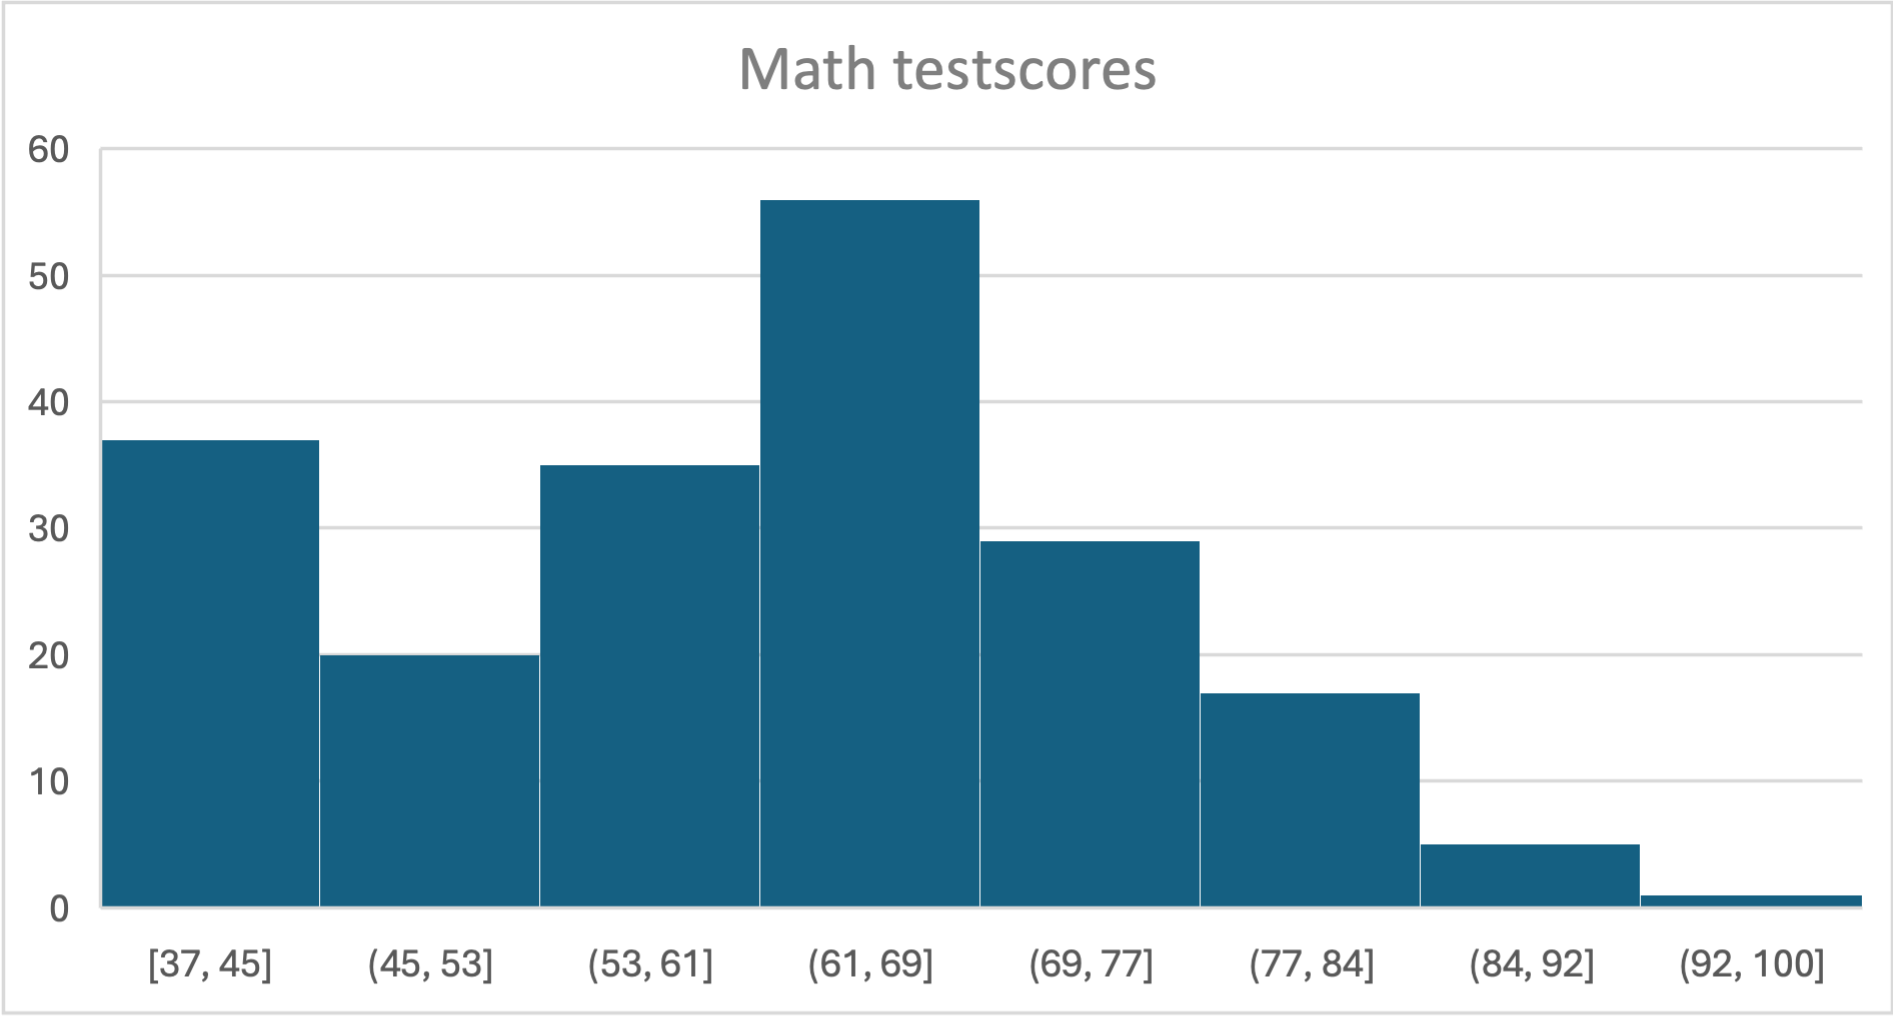
\includegraphics[width=0.45\linewidth,height=0.3\textheight]{pictures/Mathscores_hist} 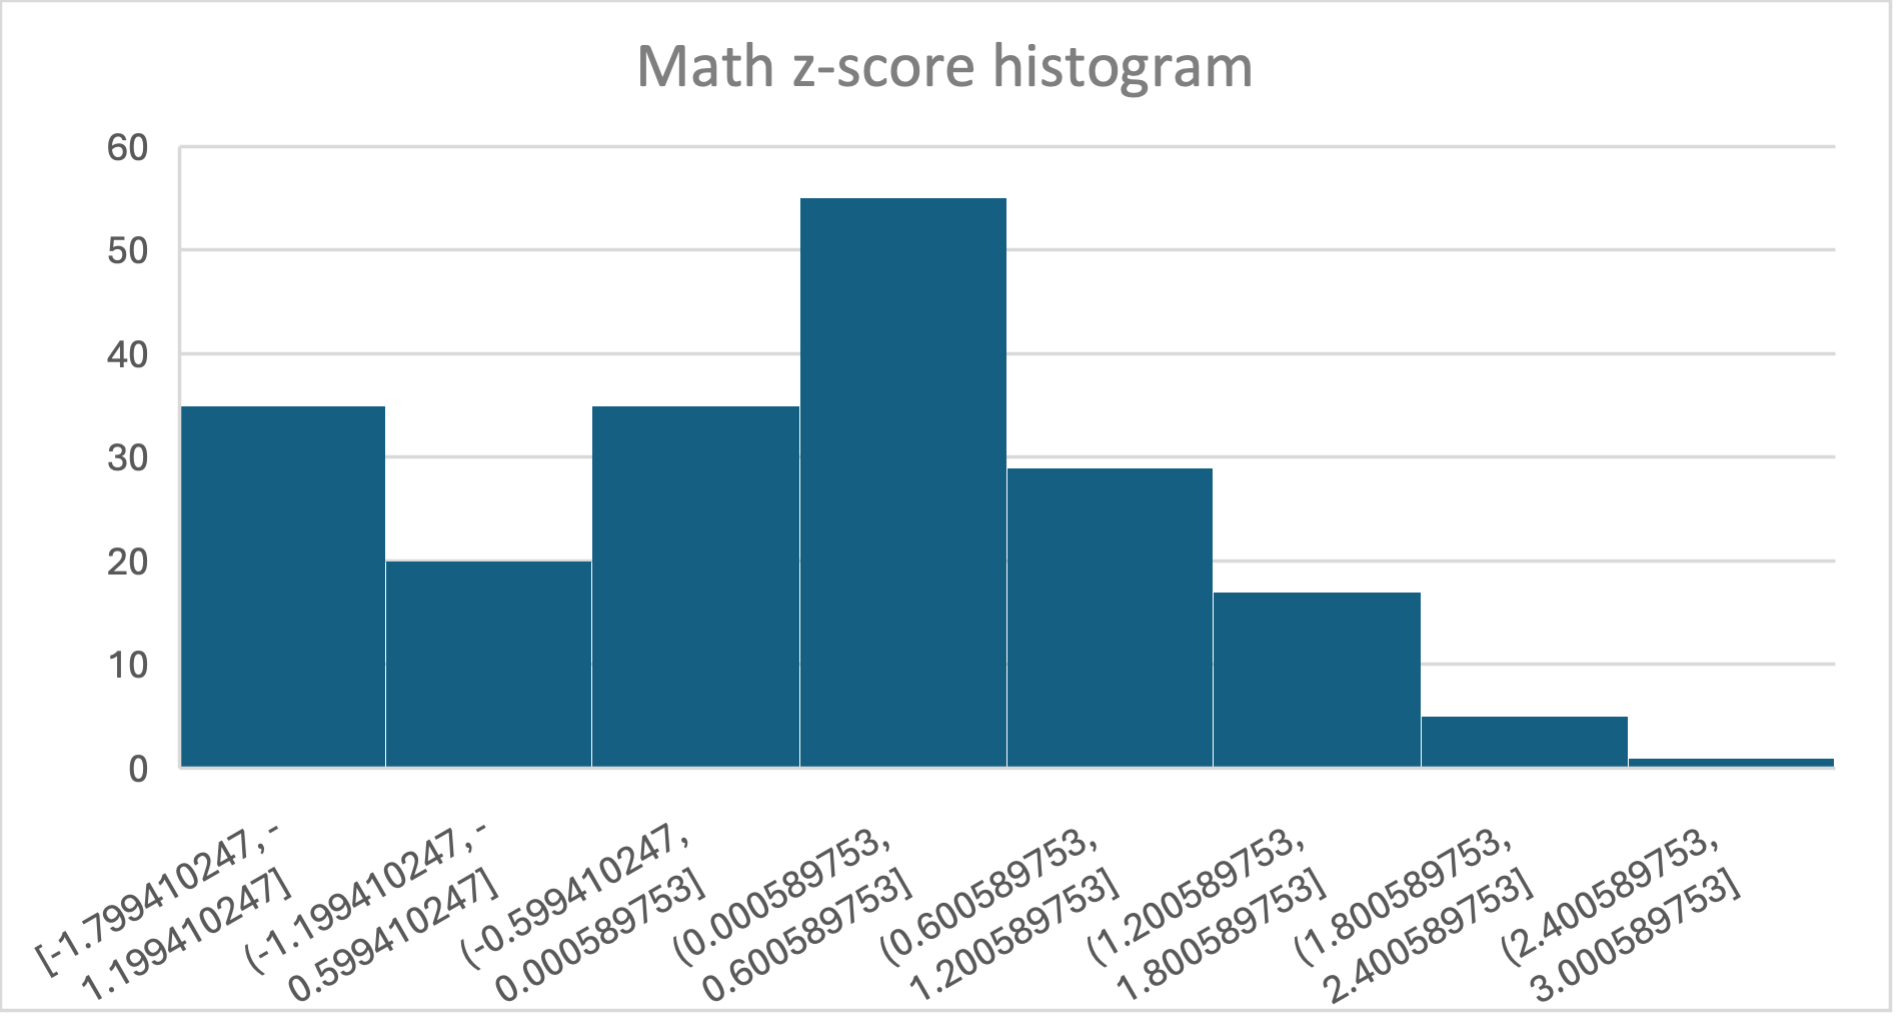
\includegraphics[width=0.45\linewidth,height=0.3\textheight]{pictures/zMathscores_hist} \end{center}
\end{frame}

\hypertarget{exercise-2.}{%
\section{Exercise 2.}\label{exercise-2.}}

\begin{frame}{Exercise 2. SE of sample mean}
\protect\hypertarget{exercise-2.-se-of-sample-mean}{}
\begin{itemize}
\tightlist
\item
  \(X\): student's test score.

  \begin{itemize}
  \tightlist
  \item
    Population standard deviation: \(\sigma_\mu\)
  \end{itemize}
\end{itemize}

\vspace{2mm}

\begin{itemize}
\tightlist
\item
  \(\bar{X}\): sample mean test score of \(n = 200\) students.

  \begin{itemize}
  \tightlist
  \item
    Standard Error of the sample mean: \(\sigma_{\bar{X}}\) \vspace{1mm}
  \item
    Sampling distribution of the sample mean \[
    \bar{X} \sim \text{Normal}(\mu,\sigma_{\bar{X}}^2) \text{ when } n \text{ is sufficient large} 
    \]
  \end{itemize}
\end{itemize}

\vspace{2mm}

\begin{itemize}
\tightlist
\item
  Formula \[
  \begin{aligned}
  \color{red}{\text{Standard Error}(\text{sample mean})} &\color{red}{=\frac{\text{Population standard deviation}}{\sqrt{\text{Sample size}}}}\\
  \color{red}{SE(\bar{X}) = \sigma_{\bar{X}}} &\color{red}{= \frac{\sigma_\mu}{\sqrt{n}}}
  \end{aligned}
  \]
\end{itemize}
\end{frame}

\begin{frame}{Exercise 2. SE of sample mean}
\protect\hypertarget{exercise-2.-se-of-sample-mean-1}{}
\begin{itemize}
\tightlist
\item
  Formula \[
  \begin{aligned}
  \text{Standard Error}(\text{sample mean}) &=\frac{\text{Population standard deviation}}{\sqrt{\text{Sample size}}}\\
  SE(\bar{X}) = \sigma_{\bar{X}} &= \frac{\sigma_\mu}{\sqrt{n}}
  \end{aligned}
  \]
\end{itemize}

\vspace{3mm}

\begin{itemize}
\tightlist
\item
  When \(\sigma_\mu\) is unknown \(\rightarrow\) Use sample standard
  deviation \(s\) instead. \[
  \widehat{SE}(\bar{X}) = \frac{s}{\sqrt{n}}
  \]
\end{itemize}
\end{frame}

\begin{frame}{Part 1. SE of sample mean (English).}
\protect\hypertarget{part-1.-se-of-sample-mean-english.}{}
We know that \(\sigma_\mu\) for variable ``English'' is equal to 4.6.

\begin{enumerate}
\tightlist
\item
  Find the sample mean for the variable ``English''.
\item
  Find the standard error of the sample mean for the variable
  ``English''.
\item
  Argue in words: What is the standard error of the sample mean useful
  for?
\end{enumerate}
\end{frame}

\begin{frame}{Part 2. SE of sample mean (Math).}
\protect\hypertarget{part-2.-se-of-sample-mean-math.}{}
We do not know \(\sigma_\mu\) for variable ``Math''.

\begin{enumerate}
\tightlist
\item
  Find the sample mean of variable ``Math''.
\item
  Find the sample standard deviation of variable ``Math'', denote as
  \(s\).
\item
  Calculate the following quantity: \[
  \widehat{SE}(\text{sample mean}) = \frac{s}{\sqrt{n}}
  \]
\end{enumerate}
\end{frame}

\hypertarget{exercise-3.}{%
\section{Exercise 3.}\label{exercise-3.}}

\begin{frame}{Part 1. If-functions.}
\protect\hypertarget{part-1.-if-functions.}{}
\begin{enumerate}
\tightlist
\item
  Create a new variable which equals 1 if the student has a math score
  above the median score.
\item
  Create a new variable which equals 1 if the student has an English
  score above the median score.
\item
  Create a new variable which equals 1 if the student has both English
  score above median and Math score above median. Call this variable
  ``high\_performer''.
\end{enumerate}

Hint: Use the \textcolor{red}{IF()} in Excel.
\end{frame}

\begin{frame}[fragile]{Part 1. If-functions.}
\protect\hypertarget{part-1.-if-functions.-1}{}
\begin{enumerate}
\tightlist
\item
  Create a new variable which equals 1 if the student has a math score
  above the median score.
  \(\color{green}{\texttt{english above median}_i = 1 \textbf{ if } \texttt{english}_i > median(\texttt{english})}\)
  \pause
\item
  Create a new variable which equals 1 if the student has an English
  score above the median score.
  \(\color{green}{\texttt{math above median}_i = 1 \textbf{ if } \texttt{math}_i > median(\texttt{math})}\)
  \pause Hint: Use the \textcolor{red}{IF()} in Excel.
\end{enumerate}

\begin{Shaded}
\begin{Highlighting}[]
\NormalTok{= IF(logical\_test,[value\_if\_true],[value\_if\_false])}
\end{Highlighting}
\end{Shaded}
\end{frame}

\begin{frame}{Part 1. If-functions.}
\protect\hypertarget{part-1.-if-functions.-2}{}
\begin{enumerate}
\setcounter{enumi}{2}
\tightlist
\item
  Create a new variable which equals 1 if the student has both English
  score above median and Math score above median. Call this variable
  ``high\_performer''.
\end{enumerate}

\small

\[
\begin{aligned}
&\color{green}{\texttt{high}\_\texttt{performer}_i = 1 \textbf{ if } \{ \texttt{english}_i > median(\texttt{english}) \textbf{ and } \texttt{math}_i > median(\texttt{math}) \} }\\
&\text{equivalently,}\\
&\color{green}{\texttt{high}\_\texttt{performer}_i = 1 \textbf{ if } \{ (\texttt{english above median}_i = 1) \textbf{ and }}\\ 
&\hspace{7cm}\color{green}{(\texttt{math above median}_i = 1) \} }
\end{aligned}
\]
\end{frame}

\begin{frame}{Part 2. Sample proportions.}
\protect\hypertarget{part-2.-sample-proportions.}{}
\begin{enumerate}
\tightlist
\item
  Calculate the sample proportion of students who have both English
  score above median and Math score above median. Interpret.
\item
  Calculate the average of variable ``high\_performer''. Interpret.
\end{enumerate}
\end{frame}

\begin{frame}{Part 3. Standard Error of Sample proportion}
\protect\hypertarget{part-3.-standard-error-of-sample-proportion}{}
We know that the population proportion of students who have above median
grades in both Math and in English is \(p = 0.29\).

\begin{enumerate}
\tightlist
\item
  Using the following formula, compute the standard error of the sample
  proportion.
\end{enumerate}

\[
SE(\text{sample proportion}) = \sigma_{\hat{p}} = \frac{\sqrt{p(p-1)}}{\sqrt{n}} = \sqrt{\frac{p(p-1)}{n}}
\]

\begin{enumerate}
\setcounter{enumi}{1}
\tightlist
\item
  Calculate the probability that \(\hat{p}\), the sample proportion of
  students with above median grades in both subjects is between \(0.25\)
  and \(0.33\).
\end{enumerate}
\end{frame}

\begin{frame}[fragile]{Part 3. Standard Error of Sample proportion}
\protect\hypertarget{part-3.-standard-error-of-sample-proportion-1}{}
\begin{enumerate}
\tightlist
\item
  Compute the standard error of the sample proportion.
\end{enumerate}

\begin{itemize}
\item
  \texttt{high\_performer} are students who have above median grades in
  both Math and in English.
\item
  Population proportion of \texttt{high\_performer}: \(p = 0.29\)
\item
  Sample proportion of \texttt{high\_performer}: \(\hat{p}\)
\item
  Verify that sample size \(n\) is large enough
  \(n \cdot p \cdot (1-p) > 5,\) which is correct as
  \(200 \cdot (0.29) \cdot (1-0.29) \approx 41.18\).
\item
  Hence, asymptotically, \[
  \hat{p} \sim \text{Normal} \left({\color{green}{p}}, {\color{red}{\frac{p(1-p)}{n}}} \right)
  \] where the Standard Error of the sample proportion is
  \(SE(\hat{p}) = \sqrt{{\color{red}{\frac{p(1-p)}{n}}}}\)
\end{itemize}
\end{frame}

\begin{frame}{Part 3. Standard Error of Sample proportion}
\protect\hypertarget{part-3.-standard-error-of-sample-proportion-2}{}
\begin{enumerate}
\setcounter{enumi}{1}
\tightlist
\item
  \(\color{blue}{P(0.25 \leq \hat{p} \leq 0.33) = ?}\)
\end{enumerate}

\normalsize

Transform \(\hat{p}\) into the standard normal random variable \(Z\)
\small \[
Z = \frac{\hat{p} - p}{SE(\hat{p})} = \frac{\hat{p} - 0.29}{SE(\hat{p})}
\] \normalsize Rewrite the probability \small \[
\begin{aligned}
P(0.25 \leq \hat{p} \leq 0.33) &= P\left(\frac{0.25 - 0.29}{SE(\hat{p})} \leq \frac{\hat{p} - 0.29}{SE(\hat{p})} \leq \frac{0.33 - 0.29}{SE(\hat{p})}\right)\\
&\overset{\text{step 1}}{=} P\left(\text{lower bound} \leq Z \leq \text{upper bound}\right)\\
&\overset{\text{step 2}}{=} P\left(Z \leq \text{upper bound}\right) - P(Z \leq \text{lower bound})\\
&\overset{\text{step 3}}{=} \text{probability (area under curve)}
\end{aligned}
\]
\end{frame}

\begin{frame}[fragile]{Part 3. Standard Error of Sample proportion}
\protect\hypertarget{part-3.-standard-error-of-sample-proportion-3}{}
\begin{enumerate}
\setcounter{enumi}{1}
\tightlist
\item
  \(\color{blue}{P(0.25 \leq \hat{p} \leq 0.33) = ?}\)
\end{enumerate}

\small

\[
\begin{aligned}
P(0.25 \leq \hat{p} \leq 0.33) &= P\left(\frac{0.25 - 0.29}{SE(\hat{p})} \leq \frac{\hat{p} - 0.29}{SE(\hat{p})} \leq \frac{0.33 - 0.29}{SE(\hat{p})}\right)\\
&\overset{\text{step 1}}{=} P\left(\text{lower bound} \leq Z \leq \text{upper bound}\right)\\
&\overset{\text{step 2}}{=} P\left(Z \leq \text{upper bound}\right) - P(Z \leq \text{lower bound})\\
&\overset{\text{step 3}}{=} \text{probability (area under curve)}
\end{aligned}
\]

Hint: Use the \textcolor{red}{NORMSDIST()} in Excel to return the
standard normal cumulative distribution

\begin{Shaded}
\begin{Highlighting}[]
\NormalTok{= NORMSDIST(z)}
\end{Highlighting}
\end{Shaded}
\end{frame}

\begin{frame}{}
\protect\hypertarget{section}{}
\begin{center}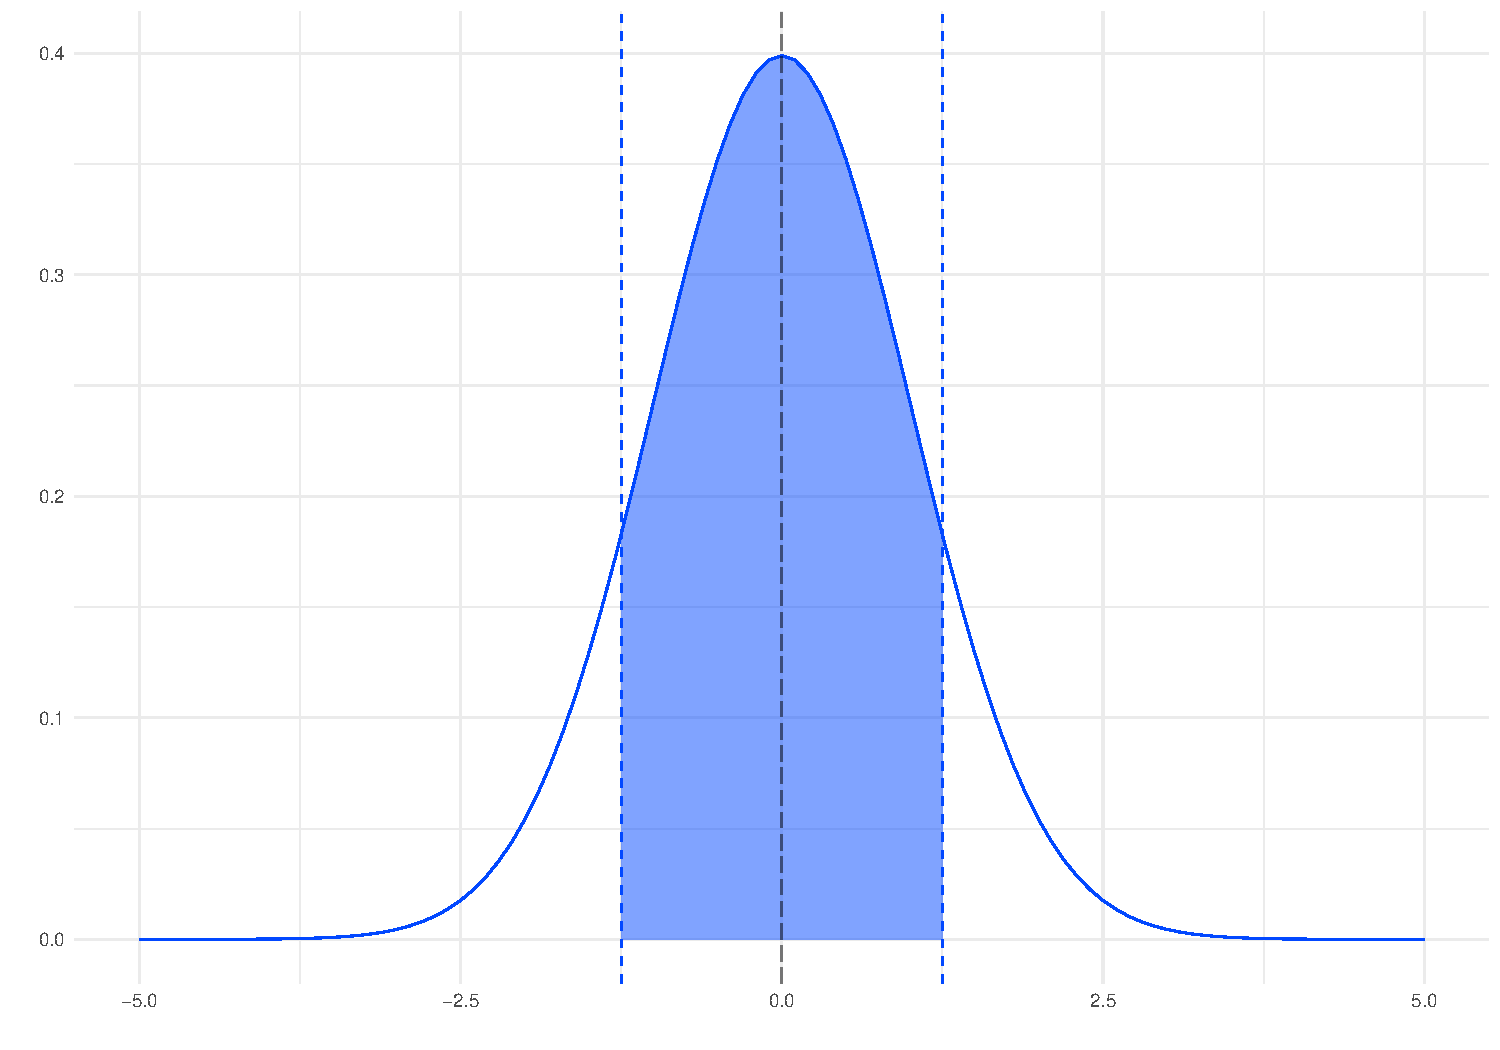
\includegraphics[width=0.5\linewidth]{ECON1013-Lab2_files/figure-beamer/unnamed-chunk-7-1} \end{center}

\begin{center}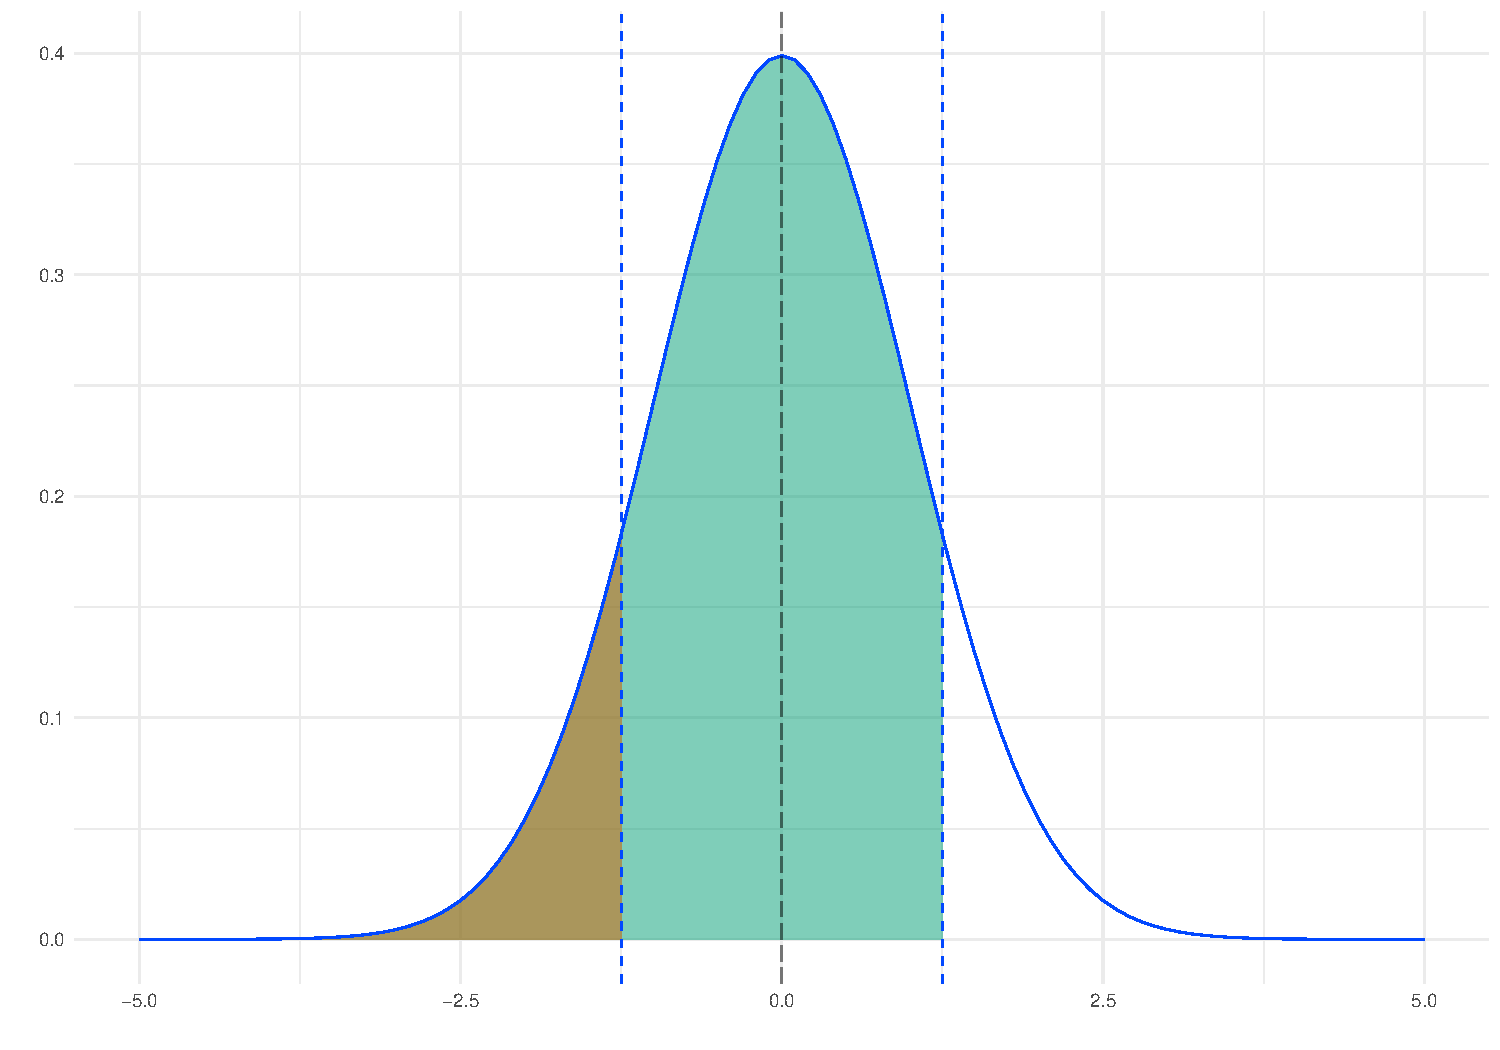
\includegraphics[width=0.5\linewidth]{ECON1013-Lab2_files/figure-beamer/unnamed-chunk-7-2} \end{center}
\end{frame}

\end{document}
